Having experimentally determined the V2PM and inverted it to obtain the P2VM, the object visibility and phase are retrieved from the experimental  data. First using the same set of data used to calibrate the V2PM and then using new ones to test the reproducibility of the method. 

The results of the retrieved phases from the data used to calibrate the V2PM matrix are shown on Fig.\ref{fig:retrieved_visi_expe}. These results aren't biased by the calibration of the V2PM because the V2PM only take into account of the visibility and phase of the output interferogram at the position of their maximum. What is flagrant from these results and the simulated ones on a similar component (see \ref{an:retrieved_visi_simu}) is that experimentally the retrieved visibility tend to oscillate a lot more around the theoretical one (expecially for baseline 14. These oscillations are mostly due to the highly overlapping output signal (as explained in the first chapter) and the delay-line being not verry accurate thus changing the coupling a little from one measurement to the other (this will be verified further). Contributions of the noise are also not negligible. With all of these imperfections the retrieve visibility are around the zone of interest (around the maximum) accurate at 10\% for the best baselines to 20\% for the worst. The visibilities retrieved on the second dataset recorded right after the calibration of the V2PM are presented on figure \ref{fig:retrieved_visi_expe2} and are far from as good as the first ones. This is mostly because of the delay-line altering the coupling in its mouvement.  


\begin{figure}[htbp!]
 \centering
 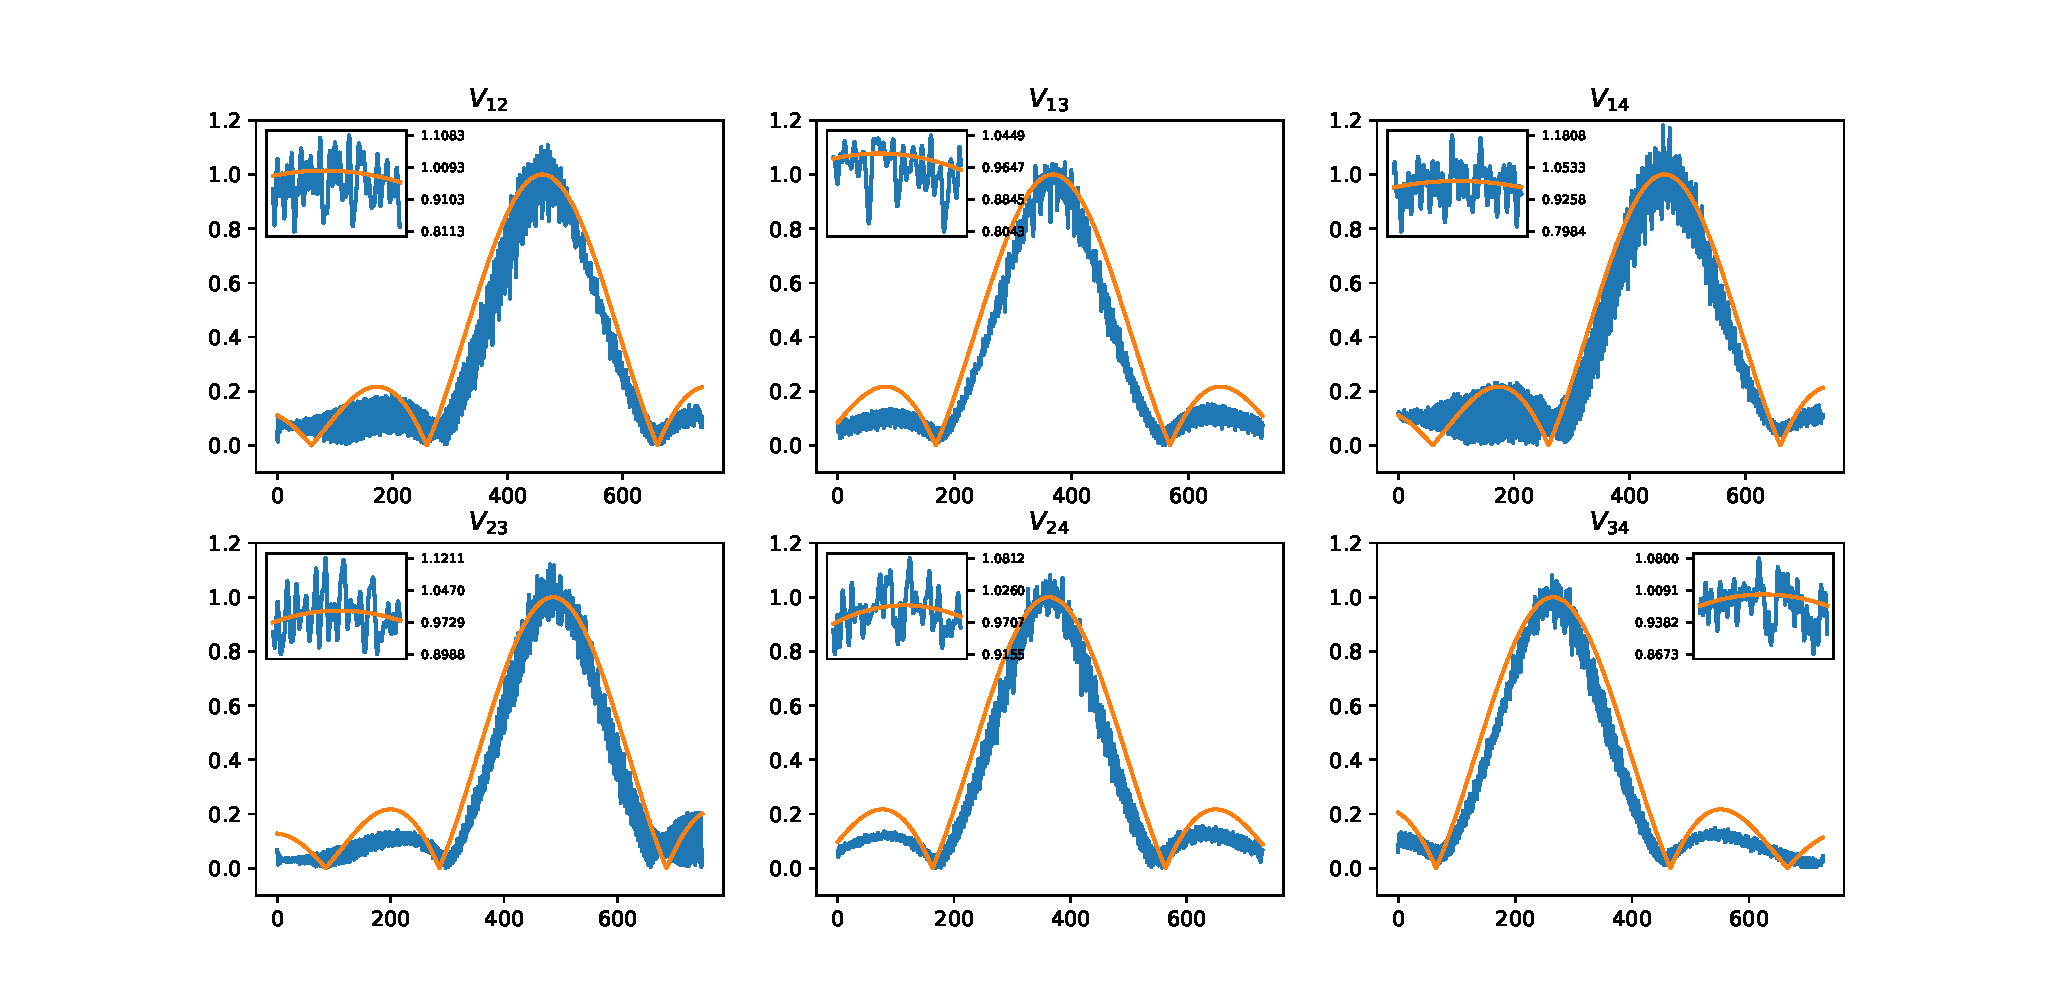
\includegraphics[scale=.45]{../picture/retrieve_visi_expe.pdf}
 \caption{Experimentally retrieved visibility from the dataset used to calibrate the V2PM. Baselines numbering 1, 2, 3, 4 refers to the input waveguides (respectively  9, 14, 10 and 19). The blue line is the actual retrieved data and the orange line the theoretical result. The inset is a zoom of the 50µm opd around the maximum. }
 \label{fig:retrieved_visi_expe}
\end{figure}

\begin{figure}[htbp!]
 \centering
 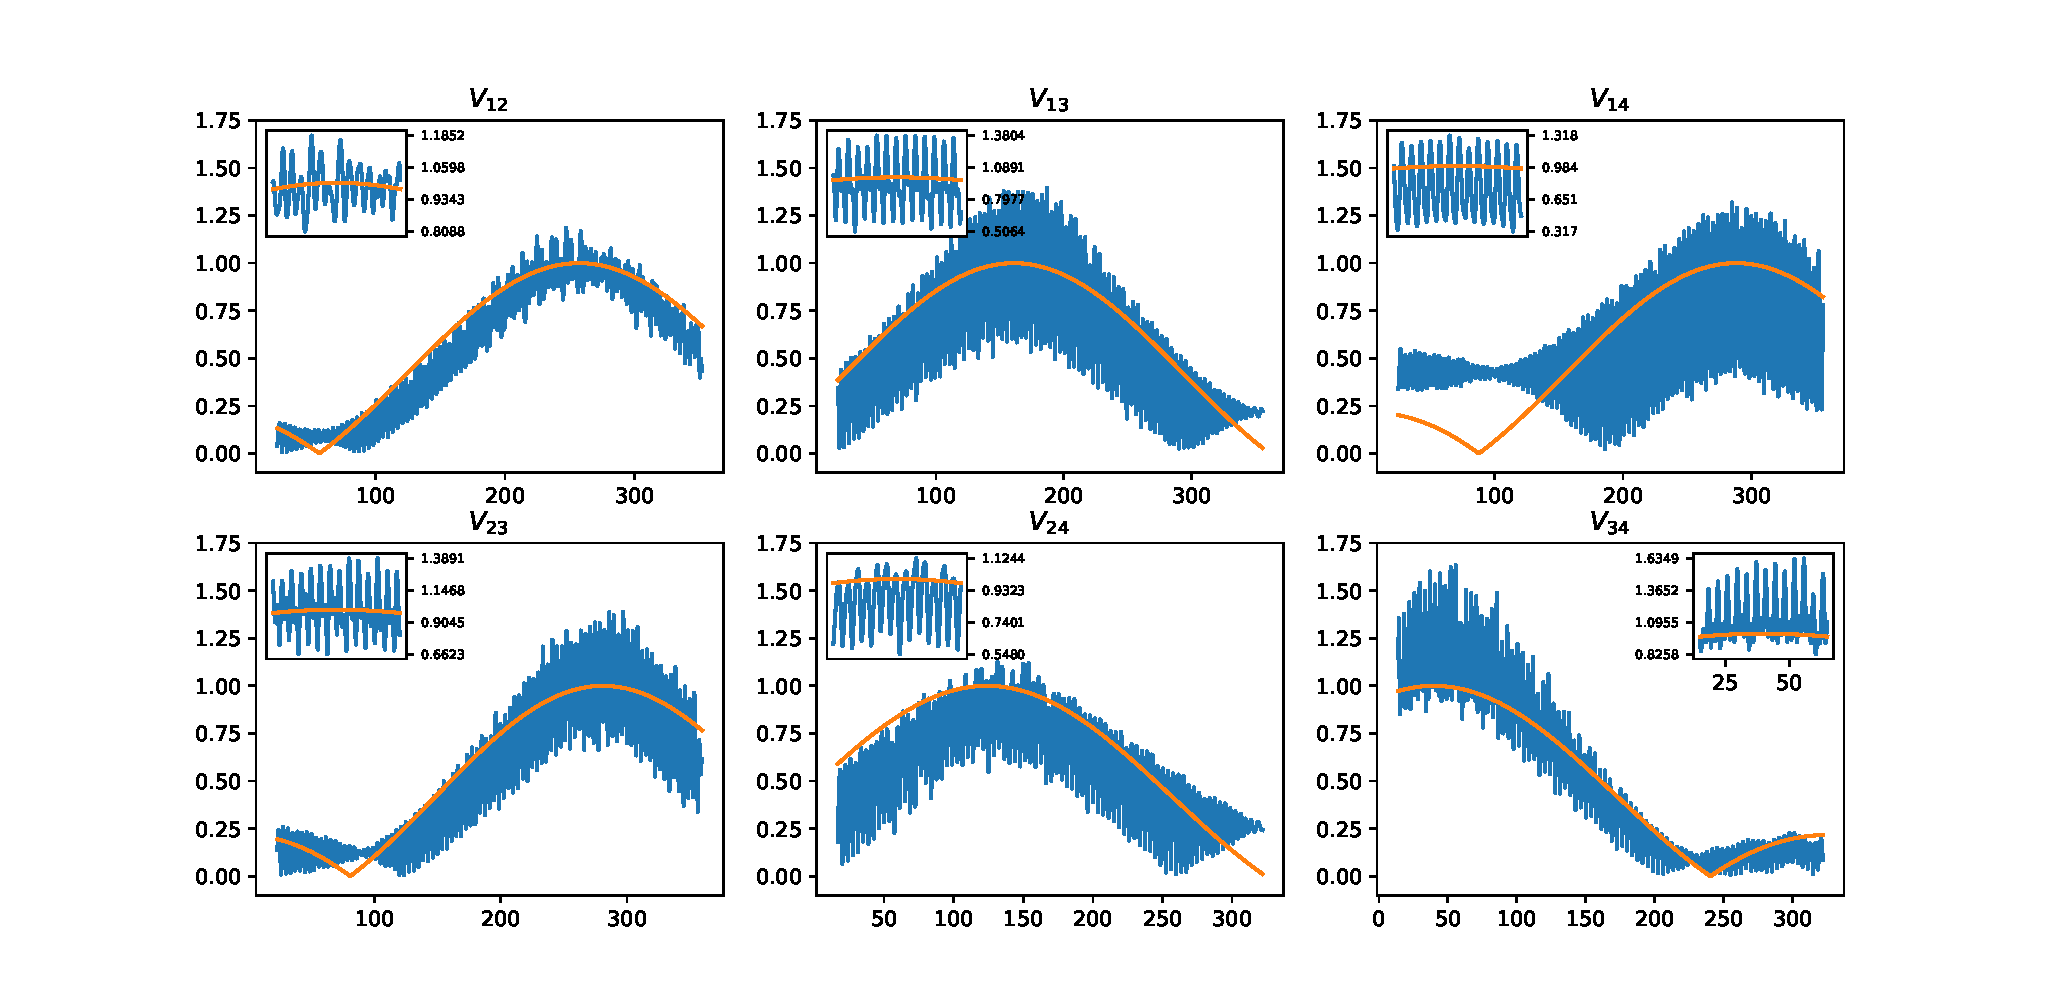
\includegraphics[scale=.45]{../picture/retrieve_visi_expe2.pdf}
 \caption{Experimentally retrieved visibility from the data recorded after the V2PM calibration. Baselines numbering 1, 2, 3, 4 refers to the input waveguides (respectively  9, 14, 10 and 19). The blue line is the actual retrieved data and the orange line the theoretical result. The inset is a zoom of the 50µm opd around the maximum. }
 \label{fig:retrieved_visi_expe2}
\end{figure}

Concerning the retrieved phase, the results are presented in Fig\ref{fig:retrieved_phase_expe} for the dataset used to calibrate the V2PM and Fig.\ref{retrieve_phase_expe2} for the second dataset zoomed around the maximum.

\begin{figure}[htbp!]
 \centering
 \includegraphics[scale=.45]{../picture/retrieve_phase_expe.pdf}
 \caption{Experimentally retrieved phase from the dataset used to calibrate the V2PM. Baselines numbering 1, 2, 3, 4 refers to the input waveguides (respectively  9, 14, 10 and 19). The blue line is the actual retrieved data and the orange line the theoretical result. }
 \label{fig:retrieved_phase_expe}
\end{figure}

\begin{figure}[htbp!]
 \centering
 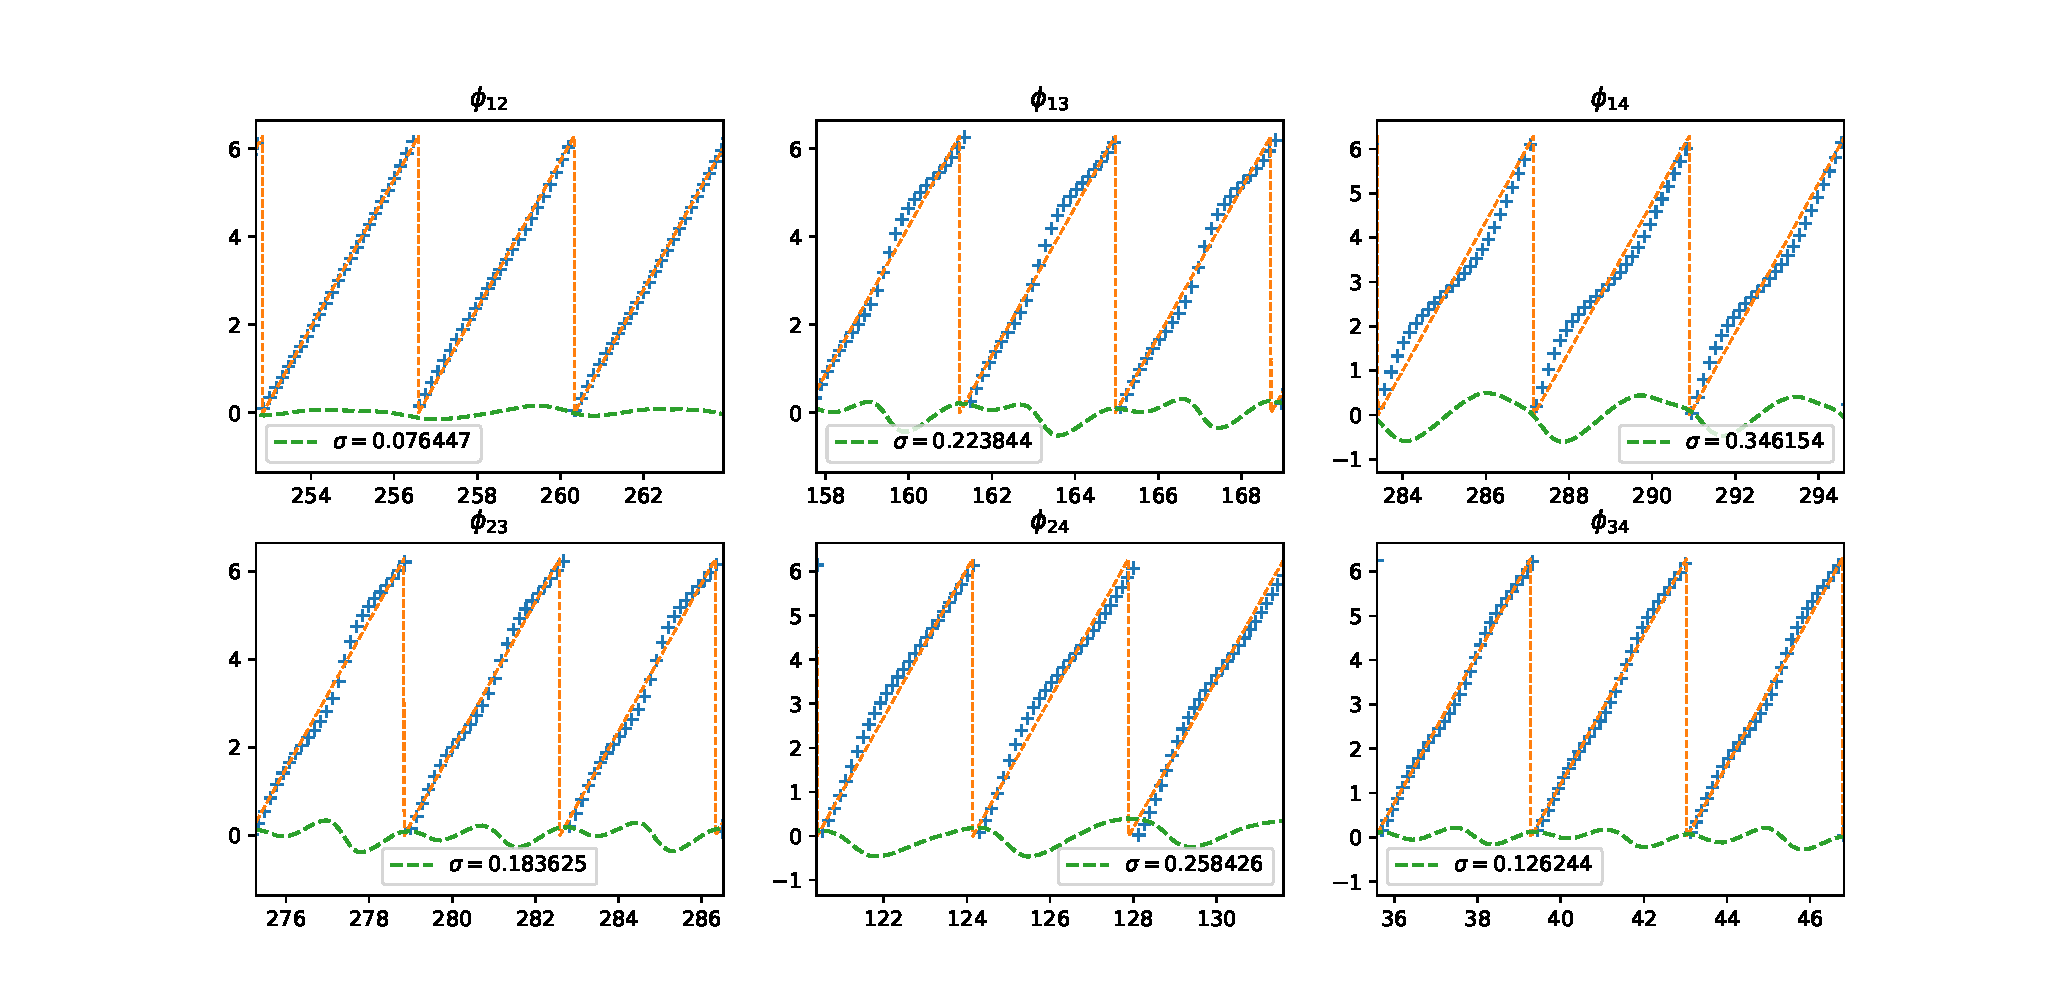
\includegraphics[scale=.45]{../picture/retrieve_phase_expe2.pdf}
 \caption{Experimentally retrieved phase from the data recorded after the V2PM calibration. Baselines numbering 1, 2, 3, 4 refers to the input waveguides (respectively  9, 14, 10 and 19). The blue line is the actual retrieved data and the orange line the theoretical result. }
 \label{fig:retrieved_phase_expe2}
\end{figure}
